\newpage
\section{PDCA}

\begin{center}
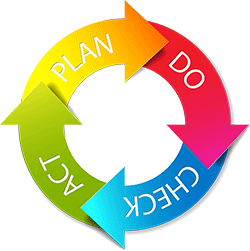
\includegraphics[keepaspectratio = true, width=5cm]{PDCA.png}
\end{center}

Il ciclo \textit{PDCA\ped{G}}, detto anche Ciclo di Deming, definisce un metodo di controllo dei processi durante il loro ciclo di vita che consente di migliorarne continuamente la qualità. \\ Tale approccio è suddiviso in 4 fasi:
\begin{itemize}
\item \textbf{Plan}: fase di pianificazione dove si individuano gli obiettivi e i processi necessari per il raggiungimento dei risultati attesi;
\item \textbf{Do}: fase di attuazione del piano individuato al passo precedente e raccolta di dati sulla qualità ottenuta;
\item \textbf{Check}: fase di verifica dove si confrontano i risultati ottenuti (fase di Do) ed i risultati attesi (fase di Plan);
\item \textbf{Act}: fase in cui si determinano le cause delle differenze fra risultati ottenuti e risultati attesi, per decidere dove attuare eventuali azioni correttive per avere un effettivo miglioramento della qualità.
\end{itemize}